\documentclass{report}

%%%%%%%%%%%%%%%%%%%%%%%%%% Practice info %%%%%%%%%%%%%%%%%%%%%%%%%%
\Subject {Системи штучного інтелекту}
\DocTitle{Логістична регресія}
\ReportType{Практична робота \#4}

%----------------------------------------------------
%	  Персональна інформація виконавця завдання
%----------------------------------------------------
\Done{Виконав:}  % Поставте правильне закінчення


\Surname{Бардін}  		% Вкажіть своє прізвище
\Name{Владислав}		% та ім'я
\Group {ІМ-42мп}     		% група в якій навчаєтесь
\YearOfStudying {1}		% курс навчання


%%%%%%%%%%%%%%%%%%%%%%%%%%%%%%%%%%%%%%%% ПОЧАТОК ЗВІТУ %%%%%%%%%%%%%%%%%%%%%%%%%%%%%%%%%%%%%%%%
\startDocument

\section{\doctitle}
\subsection{Реалізація логістичної регресії}

Реалізований код логістичної регресії наведено нижче:

\begin{lstlisting} [language=Python, style=mypython, caption={Ініціалізація вагів та зсуву}]
def parameters_inititalization(m):
  W = np.random.randn(1, m)
  b = 0.0
  return W, b
\end{lstlisting}

У функції \texttt{parameters\_initialization(m)} ми ініціалізуємо ваги \( W \) та зсув \( b \) для лінійної моделі.

\textbf{Опис:} 
Функція приймає на вхід кількість ознак \( m \), яка відповідає кількості вхідних змінних у наборі даних.

\textbf{Результат:}
\begin{itemize}
    \item \( W \) — ваги моделі, ініціалізовані випадковими малими значеннями:
    \[
    W \sim \mathcal{N}(0, \epsilon), \quad \text{де} \ \epsilon \ — \text{мала стала}.
    \]
    \item \( b \) — зсув (bias), ініціалізований нулем:
    \[
    b = 0
    \]
\end{itemize}

\begin{lstlisting} [language=Python, style=mypython, caption={Застосування нелінійної функції активації, до отриманого значення}]
def forwardPropagate(X, W, b):
  """

  z = np.dot(X, W.T) + b
  y_hat = sigmoid(z.T)
  return z.T, y_hat
  
def sigmoid(x):
  return 1 / (1 + np.exp(-x))
\end{lstlisting}

Функція \texttt{forwardPropagate(X, W, b)} обчислює лінійну комбінацію вхідних ознак та ваг, виконуючи прямий прохід моделю. 
Обчислює передбачення моделі на основі входів \( X \), ваг \( W \) та зсуву \( b \).

\textbf{Вхідні параметри:}
\begin{itemize}
    \item \( X \) — матриця розмірності \( n \times m \), де \( n \) — кількість прикладів, \( m \) — кількість ознак.
    \item \( W \) — матриця ваг моделі.
    \item \( b \) — зсув моделі (вектор розмірності \( 1 \times m \)).
\end{itemize}

\textbf{Результат:}
\begin{itemize}
    \item \( z \) — лінійна комбінація входів:
    \[
    z = WX^T + b
    \]
    \item \( \hat{y} \) — прогноз моделі після застосування сигмоїдальної функції до \( z \):
    \[
    \hat{y} = \sigma(z), \quad \text{де} \quad \sigma(z) = \frac{1}{1 + e^{-z}}
    \]
\end{itemize}

\begin{lstlisting} [language=Python, style=mypython, caption={Цільова функція}]
def cost(n, y_hat, y_true):
  ep = 10E-10
  y_hat = np.clip(y_hat, ep, 1 - ep)
  J = -(1/n) * np.sum(y_true * np.log(y_hat) + (1 - y_true) * np.log(1 - y_hat))
  return J
\end{lstlisting}

\texttt{cost(n, y\_hat, y\_true)} відповіждає за обчислює функції втрат (log-loss) для задачі класифікації.

\textbf{Вхідні параметри:}
\begin{itemize}
    \item \( n \) — кількість прикладів у наборі даних.
    \item \( y\_hat \) — передбачення моделі (ймовірності, отримані на виході моделі).
    \item \( y\_true \) — істинні значення (мітки класів, що приймають значення \( 0 \) або \( 1 \)).
\end{itemize}

\textbf{Результат:}
Функція втрат \( J \) розраховується за формулою:
\[
J = -\frac{1}{n} \sum \left( y\_true \cdot \log(y\_hat + \epsilon) + (1 - y\_true) \cdot \log(1 - y\_hat + \epsilon) \right),
\]
де \( \epsilon \) — мала додатна константа, що додається для уникнення ділення на нуль.

\begin{lstlisting} [language=Python, style=mypython, caption={Розрахунок градієнту цільвої функції відносно ваг та зсуву}]
def backwardPropagate(n, X, y_hat, y_true):
  diff = y_hat - y_true

  dW = (1/n) * np.dot(diff, X)
  db = (1/n) * np.sum(diff)

  return dW, db
\end{lstlisting}

\texttt{backwardPropagate(n, X, y\_hat, y\_true)}: Функція призначена для обчислення градієнтів, необхідних для оновлення параметрів моделі.

\textbf{Вхідні параметри:}
\begin{itemize}
    \item \( n \) — кількість прикладів у наборі даних.
    \item \( X \) — матриця вхідних даних розмірності \( n \times m \), де \( m \) — кількість ознак.
    \item \( y\_hat \) — передбачення моделі (ймовірності для кожного прикладу).
    \item \( y\_true \) — істинні мітки класів (\( 0 \) або \( 1 \)).
\end{itemize}

\textbf{Результат:}
\begin{itemize}
    \item \( dW \) — градієнт функції втрат за вагами \( W \):
    \[
    dW = \frac{1}{n} \cdot (y\_hat - y\_true)^T \cdot X
    \]
    \item \( db \) — градієнт функції втрат за зсувом \( b \):
    \[
    db = \frac{1}{n} \cdot \sum (y\_hat - y\_true)
    \]
\end{itemize}

\begin{lstlisting} [language=Python, style=mypython, caption={Оновлення ваг та зсуву}]
def update(lr, dW, db, W, b):
  W = W - lr * dW
  b = b - lr * db

  return W, b
\end{lstlisting}

Функція \texttt{update(lr, dW, db, W, b)} оновлює параметри моделі \( W \) та \( b \) за допомогою алгоритму градієнтного спуску.

\textbf{Вхідні параметри:}
\begin{itemize}
    \item \( lr \) — швидкість навчання (learning rate), що визначає розмір кроку оновлення параметрів.
    \item \( dW \) — градієнт функції втрат за вагами \( W \).
    \item \( db \) — градієнт функції втрат за зсувом \( b \).
    \item \( W \) — поточні ваги моделі.
    \item \( b \) — поточний зсув моделі.
\end{itemize}

\textbf{Результат:}
Оновлені параметри \( W \) та \( b \), обчислені за наступними формулами:
\[
W = W - lr \cdot dW
\]
\[
b = b - lr \cdot db
\]

\subsection{Тестування логістичної регресії}

Для тестування скористаємось наступним кодом.

\begin{lstlisting} [language=Python, style=mypython, caption={Розрахунок градієнту цільвої функції відносно ваг та зсуву}]
np.random.seed(1)

learning_rates = [0.001, 0.005, 0.01, 0.05, 0.1]
iterations = [100, 500, 1000, 1500, 2000, 2500, 3000, 4500]
results = []

fig = plt.figure(figsize=(10, 8))

for lr in learning_rates:
    costs_over_iterations = []

    for n_iters in iterations:
        model = LogisticRegression(lr=lr, n_iters=n_iters)
        model.fit(X_train, y_train)

        cost_value = model.evaluate(X_test, y_test)
        costs_over_iterations.append(cost_value)

        results.append({
            "Learning Rate": lr,
            "Iterations": n_iters,
            "Cost": cost_value
        })

    plt.plot(iterations, costs_over_iterations, label=f"LR={lr}")

plt.title("Change in model losses with respect to the number of iterations")
plt.xlabel("Number of iterations")
plt.ylabel("Losses")
plt.legend(title="Learning Rate")
plt.grid(True)
plt.show()
\end{lstlisting}

\begin{figure}
    \centering
    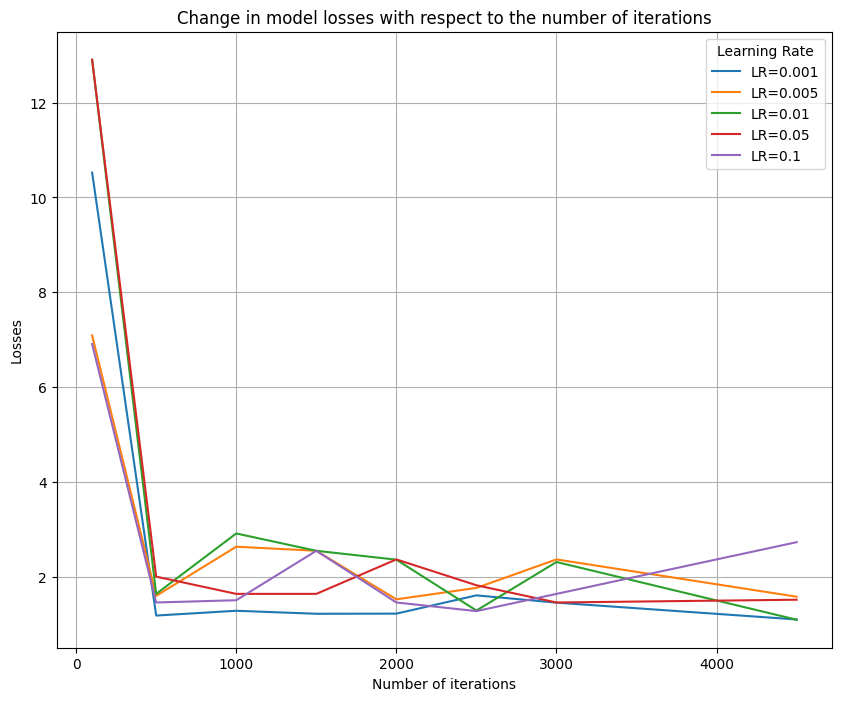
\includegraphics[width=1\linewidth]{fig1.png}
    \caption{Зміни втрат відносно кількості ітерацій}
    \label{fig:enter-label}
\end{figure}

\newpage
Графік демонструє зміну втрат моделі (losses) залежно від кількості ітерацій для різних значень швидкості навчання (learning rate). На основі отриманих даних можна зробити наступні висновки:

\begin{itemize}
    \item \textbf{Швидкість навчання (\( \text{LR} = 0.1\))}: 
    Найвищі значення швидкості навчання показують нестабільну поведінку моделі. Незважаючи на швидкий початковий спад втрат, модель починає демонструвати коливання втрат при збільшенні кількості ітерацій. Це свідчить про те, що занадто велика швидкість навчання може призвести до переосциляцій і ускладнень в оптимізації.
    
    \item \textbf{Швидкість навчання (\( \text{LR} = 0.05\))}: 
    Помірне значення швидкості навчання демонструє кращу стабільність, але також може викликати деякі коливання при більшій кількості ітерацій. Це свідчить про те, що обране значення \( \text{LR} = 0.05 \) є допустимим, але потребує додаткового налаштування.

    \item \textbf{Швидкість навчання (\( \text{LR} = 0.01 \) і \( \text{LR} = 0.005 \))}: 
    Ці значення швидкості навчання демонструють найбільш стабільне зниження втрат без суттєвих коливань. Втрати поступово зменшуються зі збільшенням кількості ітерацій, що свідчить про ефективність цих параметрів для навчання моделі.

    \item \textbf{Швидкість навчання (\( \text{LR} = 0.001 \))}: 
    Найменше значення швидкості навчання демонструє стабільну, але дуже повільну збіжність. Це свідчить про те, що зменшення швидкості навчання надмірно уповільнює процес оптимізації, що може бути неприйнятним у багатьох практичних застосуваннях.

\end{itemize}

Вибір швидкості навчання є критично важливим для стабільного та ефективного навчання моделі. Надто велика швидкість (\( \text{LR} = 0.1 \)) може спричинити нестабільність, тоді як надто мала (\( \text{LR} = 0.001 \)) значно уповільнює процес. Оптимальними значеннями для цієї задачі виглядають \( \text{LR} = 0.01 \) та \( \text{LR} = 0.005 \), які забезпечують як стабільність, так і ефективну збіжність.


\newpage
\section{Висновки}
У ході виконання роботи було реалізовано тестування алгоритму логістичної регресії з різними значеннями швидкості навчання (\( \text{LR} \)) та кількості ітерацій. Проведено аналіз впливу цих параметрів на зниження втрат (losses) та стабільність моделі.

Оптимальним значенням швидкості навчання виявилося \( \text{LR} = 0.005 \), яке забезпечує стабільне зниження втрат без суттєвих коливань. При значенні \( \text{LR} = 0.01 \) спостерігалися незначні коливання втрат після 2000 ітерацій, що вказує на ймовірну нестабільність моделі при подальшому збільшенні кількості ітерацій.

Для значення \( \text{LR} = 0.1 \) було зафіксовано швидкий початковий спад втрат, однак модель демонструвала нестабільність і значні коливання втрат при збільшенні ітерацій. Навпаки, при \( \text{LR} = 0.001 \) модель показала стабільність, але швидкість навчання виявилася надто низькою, що значно уповільнило процес оптимізації.

Також було помічено, що після 3000 ітерацій втрати починають зростати для деяких значень \( \text{LR} \), тому доцільно застосовувати метод раннього завершення навчання (early stopping).

Загалом, алгоритм демонструє хорошу ефективність у задачах класифікації за умови правильного налаштування швидкості навчання та використання механізмів стабілізації, таких як раннє завершення навчання.

\end{document}
